\chapter{Ownership, Cost, and the Discipline of Scale}

This lecture begins with spectacle: giant revenue figures, famous names, and a city announced as richer than most countries. But the durable content comes later. As the host moves from failed street approaches to four substantive conversations, wealth becomes legible through a small number of recurring mechanisms: ownership of the asset, control of the cost base, the ability to recruit help and survive failure, and the discipline of taking the next step under pressure. The mathematics here is not classroom mathematics. It is the arithmetic of catalogs, advances, margins, debt, horizons, and cumulative action.

\section{New York as a Field of Wealth}

The opening montage gives us wealth in its most compressed form: billionaires, celebrity founders, the mayor of New York, and revenues large enough to provoke disbelief. Then the lecture slows down and tells us what it is actually going to do. New York is not merely a backdrop. It is the field in which wealth is visible while explanation remains scarce.

The first substantive movement is failure. The host stops people on the street, and the answers are partial, evasive, or private. One man says he was ``born in the right place.'' Another says he is not a public person. This matters. Before we get a model of wealth, we get a model of access. Riches may be concentrated, but their explanations are not handed out freely.

That is why the pivot to Tribeca matters. The lecture changes geography in order to change the probability of finding a speaker who will move past status and into mechanism. The shift is not decorative. It is the condition for the first real piece of business arithmetic.

\section{Owning the Music, Not Just Making It}

In Tribeca the lecture finds Russ, and with him the first clean mechanism. The surprise is immediate: a musician can make roughly \$25 million in a year. The explanation is equally immediate: most musicians are not poor because music lacks money. They are poor because they do not own the thing that produces the money.

\begin{definition}
In the vocabulary of this lecture, the \emph{master} is the owned recording itself. It is the asset that carries the claim on future revenue. To give away the master is to give away the revenue-bearing object.
\end{definition}

Once that point is fixed, the rest of the section follows almost mechanically. If a musician owns a large enough catalog, total income no longer depends on one hit alone. It becomes a sum over many owned assets:
\begin{equation}
I_{\mathrm{catalog}}=\sum_{i=1}^{N} I_i,\qquad N\approx 500+.
\end{equation}
The transcript gives only an approximate count, but the logic is exact enough. One song may fail to produce life-changing money. Hundreds of owned songs can change the problem from fragility to accumulation.

Russ's phrasing is important here. He does not say, ``I need one song to make me a million dollars.'' He says he can have many songs each making some smaller amount. That is a diversification argument, even though it is made in the language of music rather than portfolio theory.

\subsection{Question \& Answer}

\paragraph{Question.} If music makes money, why are so many musicians broke?

\paragraph{Answer.} Because the artist and the asset are not the same thing. The lecture makes this explicit through a simple recoupment example. A label advances money up front, but that advance is not free income. It is a threshold that future music revenue must first repay:
\begin{align}
A &= \$2\,\mathrm{M},\\
R_{\mathrm{music}}<A &\Longrightarrow n_{\mathrm{checks}}=0,\\
R_{\mathrm{music}}\ge A &\Longrightarrow R_{\mathrm{artist}}\approx \frac{1}{2}\bigl(R_{\mathrm{music}}-A\bigr).
\end{align}
Here \(A\) is the advance, \(R_{\mathrm{music}}\) is the cumulative revenue returned by the music, and \(n_{\mathrm{checks}}\) is the number of later royalty checks in the lecture's simplified illustration. The split after recoupment is not a universal contract formula; it is Russ's stripped-down explanatory model. But it is enough for the point at hand.

The point is this. If the artist never earns back the advance, then the advance has already been spent, the artist remains unrecouped, and the promised future checks never arrive. If the artist does recoup, the money begins to flow only after the threshold has been crossed, and then it flows only on the timetable the label uses. Russ summarizes that timetable in plain language: two checks a year.

\begin{figure}
\centering
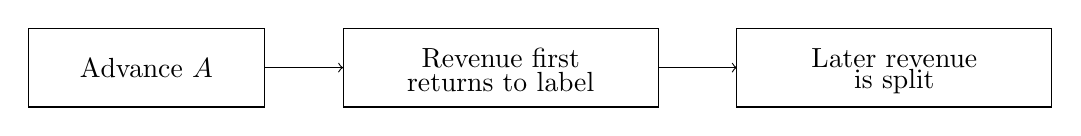
\begin{tikzpicture}[x=1cm,y=1cm]
\draw (0,0) rectangle (3,1);
\node at (1.5,0.5) {Advance \(A\)};
\draw[->] (3,0.5) -- (4,0.5);
\draw (4,0) rectangle (8,1);
\node at (6,0.62) {Revenue first};
\node at (6,0.32) {returns to label};
\draw[->] (8,0.5) -- (9,0.5);
\draw (9,0) rectangle (13,1);
\node at (11,0.62) {Later revenue};
\node at (11,0.32) {is split};
\end{tikzpicture}
\caption{A transcript-backed reconstruction of the recoupment mechanism described by Russ.}
\end{figure}

This is why the lecture insists so strongly that ``the money is in music'' and then sharpens the claim: the money is in \emph{owning} the music. Labels themselves are the proof. They do not need to tour in order to make money from the owned recordings.

\section{Patience, Public Opinion, and the Artist's Cash-Flow Machine}

Once ownership is established, the lecture widens from structure to temperament. Russ says he has turned down \$50 million for the rights to his music. Here the argument is no longer only contractual. It becomes moral and temporal. He calls such a sale a form of selling the soul, because the music is not merely a product but an extension of the self. Whether or not we adopt the moral language, the economic structure is clear enough: the lump sum competes against a long future of owned cash flow.

That transition leads naturally to time. Russ's line that ``faith requires more than 48 hours'' is really a statement about evaluation horizons. A creative work cannot be judged on the smallest clock alone. The lecture thus moves from a weekly panic to a decade-scale patience:
\begin{equation}
48\,\mathrm{hours}<1\,\mathrm{week}<1\,\mathrm{year}<2\,\mathrm{years}<10\,\mathrm{years}.
\end{equation}
This is not mystical notation. It is a ranking of time windows. It says: if we evaluate too early, we systematically misread the value of the work.

The lecture then gives a concrete reinvestment example. Russ says that his best investment is the music itself, and he illustrates the claim with a song that cost about \$9.99 to upload and later made about \$2 million.

\paragraph{Worked example.} If we formalize only the arithmetic stated in the interview, we get
\begin{align}
C_{\mathrm{song}} &\approx \$9.99,\\
R_{\mathrm{song}} &\approx \$2{,}000{,}000,\\
\frac{R_{\mathrm{song}}}{C_{\mathrm{song}}} &\sim 2\times 10^5.
\end{align}
The lecture does not present audited net profit. It presents an anecdotal gross return. But as an order-of-magnitude statement the example is powerful. The artist's highest-return asset is the thing he already knows how to make and, crucially, still owns.

\subsection{Question \& Answer}

\paragraph{Question.} How do we survive hate in a business where public feeling is part of the revenue model?

\paragraph{Answer.} The lecture answers with a distinction between finite performance and approval-dependent performance. In sports, Russ says, a player can average \(25\), \(10\), and \(6\), and those are finite numbers. The contract follows the stat line. In music, public feeling enters directly into livelihood. We can schematically write the contrast as
\begin{equation}
\mathbf{s}_{\mathrm{sport}}=(25,10,6),\qquad I_{\mathrm{music}}=I\!\left(P_{\mathrm{public}}\right),
\end{equation}
where \(P_{\mathrm{public}}\) is not a box score but a floating social variable: taste, reputation, likeability, mood, identification.

The lecture refuses the comforting slogan that artists should not care what anyone thinks. In this line of work, what people think does, quite literally, pay the bills. But the answer is not paralysis. It is iteration. If the public variable is unstable, then the artist's job is to keep putting new work into the world. Russ's answer is blunt and operational: drop your way through it. Keep releasing songs.

At the end of this conversation the lecture briefly slides from business into appetite and self-government. That material is not algebraic, but it remains structurally relevant. A catalog can grow only if the person making it does not repeatedly sabotage the production process.

\section{Price Power without Debt: The Arizona Machine}

The move from Russ to Don Vultaggio is a deliberate change of texture. We leave the world of intangible rights and enter the world of trucks, factories, cans, shelves, and fuel. The lecture now asks a different question: how can a consumer product remain cheap for decades without destroying itself?

Don's biographical opening matters. No family money, no college, truck driving, gradual expansion. Then comes the cautionary memory of A\&P, once enormous and later gone:
\begin{equation}
S_{\mathrm{A\&P}}:15000\to 0.
\end{equation}
The lecture uses this not as retail history for its own sake, but as a warning: scale does not save a business that forgets the customer.

From there the chapter turns to Arizona's famous retail number, \$0.99, and asks how such pricing survived inflation, freight shocks, and general cost pressure.

\subsection{Question \& Answer}

\paragraph{Question.} How can a \(99\)-cent product survive inflation for decades?

\paragraph{Answer.} Don's answer is that price is inseparable from capital structure. We write the unit-profit identity in its simplest form:
\begin{equation}
\Pi=(p-c)q,\qquad p=\$0.99.
\end{equation}
If we are going to hold \(p\) down, then we must control \(c\), the unit cost. The lecture then decomposes that cost into the pieces it cares about:
\begin{equation}
c=c_{\mathrm{operations}}+c_{\mathrm{distribution}}+c_{\mathrm{interest}}.
\end{equation}
The essential claim is that Arizona removes the financing term:
\begin{equation}
c_{\mathrm{interest}}=0.
\end{equation}
Buildings are owned. Factories are owned. Equipment is owned. The company owes neither a bank nor a board a mandatory price increase. Once this is seen, the \(99\)-cent can is no longer a miracle. It is a consequence of ownership and a refusal to serve debt.

\paragraph{Worked derivation.} The lecture's logic can be written as a short chain.
\begin{enumerate}
\item Keep the retail price fixed at \(p=\$0.99\).
\item Remove financing drag by setting \(c_{\mathrm{interest}}=0\).
\item Reduce pressure on the margin \(p-c\).
\item Accept that the per-unit margin may still be tight.
\item Increase total sales \(q\) so that volume offsets some of the lower margin.
\end{enumerate}
This is precisely Don's answer when the host asks whether he prioritizes reach over margins. Margins matter, but increased sales can make up for lost margin.

The lecture adds one more number to this picture. A new New Jersey factory was built for more than \$400 million and paid for in cash:
\begin{equation}
K_{\mathrm{factory}}>\$4\times 10^8.
\end{equation}
This is retained-capital optionality in its starkest form. The point is not only that the business is profitable. It is that the business has accumulated enough internal capital to buy strategic flexibility.

\begin{figure}
\centering
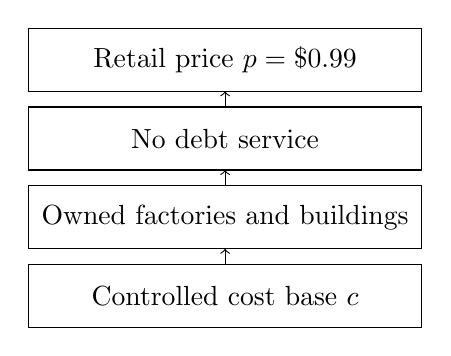
\begin{tikzpicture}[x=1cm,y=1cm]
\draw (0,0) rectangle (5,0.8);
\node at (2.5,0.4) {Retail price \(p=\$0.99\)};
\draw (0,-1) rectangle (5,-0.2);
\node at (2.5,-0.6) {No debt service};
\draw (0,-2) rectangle (5,-1.2);
\node at (2.5,-1.6) {Owned factories and buildings};
\draw (0,-3) rectangle (5,-2.2);
\node at (2.5,-2.6) {Controlled cost base \(c\)};
\draw[->] (2.5,-0.2) -- (2.5,0);
\draw[->] (2.5,-1.2) -- (2.5,-1);
\draw[->] (2.5,-2.2) -- (2.5,-2);
\end{tikzpicture}
\caption{A transcript-backed cost-stack sketch for Arizona: price stability is supported from below by ownership and debt avoidance.}
\end{figure}

The rest of the Don interview sharpens this picture. First, packaging is not decoration but acquisition. In a beverage business, if incumbents can outspend us in conventional advertising, then the container itself must function as the first advertisement. Second, operational modernization matters. The business roughly doubled in ten years without doubling staff, so the productivity ratio must have improved:
\begin{equation}
Y_{10}\approx 2Y_0,\qquad L_{10}<2L_0
\quad\Longrightarrow\quad
\left(\frac{Y}{L}\right)_{10}>\left(\frac{Y}{L}\right)_0.
\end{equation}
The lecture does not give exact output units, and it does not need to. The direction of the change is enough.

At one point Don reduces entrepreneurial accounting to a nearly primitive law: know your costs and sell above them. The statement is not sophisticated, but neither is it childish. Underneath the whole Arizona section lies the conviction that many firms fail because they do not actually know what their own unit economics are.

\begin{remark}
The video briefly pauses here for a promotional interlude about the host's membership community. Since it does not add a new mechanism of wealth construction, we set it aside and return to the main chain of arguments.
\end{remark}

\section{Rebuilding from Zero: Voids, People, and Relationship Capital}

Michael Rubin brings the lecture back to scale. Fanatics is said to be around \$12 billion in revenue, employs roughly \(22{,}000\) people, and is valued at around \$25 billion:
\begin{equation}
R_{\mathrm{Fanatics}}\approx \$12\times 10^9,\qquad
L_{\mathrm{Fanatics}}=22000,\qquad
V_{\mathrm{Fanatics}}\approx \$25\times 10^9.
\end{equation}
But the lecture does not stay long with sheer size. It immediately converts the numbers into a more interesting question: if everything disappeared tomorrow, how would we rebuild?

\subsection{Question \& Answer}

\paragraph{Question.} What are the first moves if we had to rebuild a billion-dollar company from scratch?

\paragraph{Answer.} Rubin gives the cleanest operator sequence in the lecture:
\begin{equation}
\text{study}\to\text{find void}\to\text{sprint}\to\text{get the right people}\to\text{iterate after failure}.
\end{equation}
This is the blueprint as he states it. It begins not with capital but with attention. Study the field until an absence becomes visible. Then move quickly. But speed alone is insufficient. The process is social. Get the right people because no large build is a solo act. If the attempt fails, run the operator again.

\begin{figure}
\centering
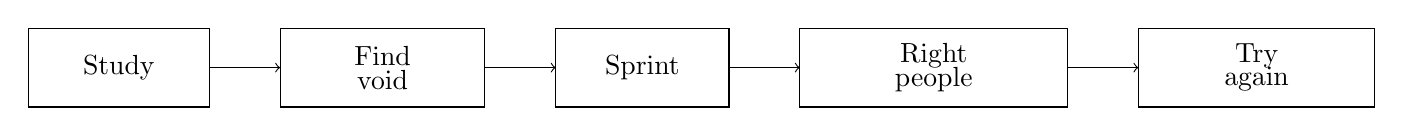
\begin{tikzpicture}[x=1cm,y=1cm]
\draw (0,0) rectangle (2.3,1);
\node at (1.15,0.5) {Study};
\draw[->] (2.3,0.5) -- (3.2,0.5);
\draw (3.2,0) rectangle (5.8,1);
\node at (4.5,0.65) {Find};
\node at (4.5,0.35) {void};
\draw[->] (5.8,0.5) -- (6.7,0.5);
\draw (6.7,0) rectangle (8.9,1);
\node at (7.8,0.5) {Sprint};
\draw[->] (8.9,0.5) -- (9.8,0.5);
\draw (9.8,0) rectangle (13.2,1);
\node at (11.5,0.65) {Right};
\node at (11.5,0.35) {people};
\draw[->] (13.2,0.5) -- (14.1,0.5);
\draw (14.1,0) rectangle (17.1,1);
\node at (15.6,0.65) {Try};
\node at (15.6,0.35) {again};
\end{tikzpicture}
\caption{A transcript-backed reconstruction of Rubin's rebuild-from-zero sequence.}
\end{figure}

Rubin then adds the social infrastructure beneath that sequence. Relationships do not matter much in good times, he says, but in bad times they matter enormously. That is a sharper claim than ordinary networking advice. It means that relationships are not ornaments of success. They are bridges across failure.

This is why the lecture keeps pressing on help. The right people help not merely by joining the company but by extending time, trust, and rescue across a period in which the system might otherwise fail. When Rubin names Robert Kraft and Jonathan Kraft, the argument is not celebrity worship. It is an argument about mentorship as an input to institutional growth.

The same rhythm appears in his account of failure. Broke at fifteen, creditors at the door, then a rapid rise a few years later to roughly \$100 million in sales and \$10 million in annual earnings by age twenty-one in what the transcript garbles as the ``close-up'' business. The sector label is uncertain, but the numerical sequence is not. His point is that losses do not invalidate the process. They train it.

That claim leads naturally to horizon length. The host mentions the one-year question. Rubin rejects it. A decade is already short for him. The lecture's order relation is simple:
\begin{equation}
1\,\mathrm{year}<10\,\mathrm{years}<\text{lifetime horizon}.
\end{equation}
The strongest version of the point is not that long-term thinking is noble. It is that short-term thinking systematically produces avoidable mistakes, while lifetime thinking changes the objective function from immediate extraction to durable belovedness.

\section{One Day at a Time Under Public Pressure}

The last movement of the lecture leaves private wealth and moves into public responsibility. Eric Adams is not presented as a business founder but as the executive of a city. The arithmetic changes accordingly:
\begin{equation}
N_{\mathrm{people}}=8.5\times 10^6,\qquad
N_{\mathrm{opinions}}=3.5\times 10^7.
\end{equation}
The second number is rhetorical, but that is part of its use. It dramatizes the mismatch between a finite office and an effectively unbounded noise field.

Adams first answers pressure with proportion. New Yorkers will judge, mock, and criticize, so one must not let the noise become the governing variable. Then the lecture turns inward. Dyslexia, ridicule, bullying, compensating systems, and the re-reading of dark places not as burials but as plantings. This is the most explicitly therapeutic section of the chapter, but it still has structure. A bad beginning can function as preparation rather than negation.

\subsection{Question \& Answer}

\paragraph{Question.} What is the first actionable step when we are at rock bottom?

\paragraph{Answer.} Adams's answer is a discrete-time process. We do not begin by conquering the whole future. We begin by executing the smallest next move:
\begin{equation}
s_1=\text{get out of bed},\qquad
s_2=\text{shower/change clothes},\qquad
s_3=\text{repeat tomorrow}.
\end{equation}
The lecture's logic is cumulative. Small successes make the next small successes easier. Once repeated, they cease to require deliberation. That is why Adams can say that the process fails only when the next step is not taken.

\begin{figure}
\centering
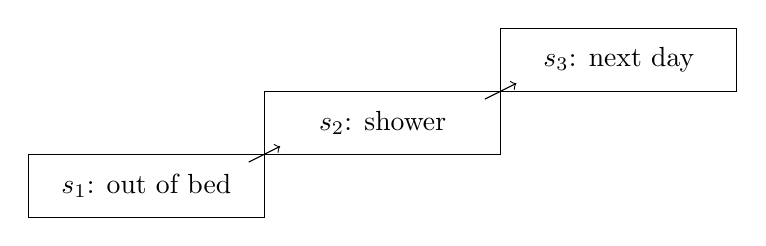
\begin{tikzpicture}[x=1cm,y=1cm]
\draw (0,0) rectangle (3,0.8);
\node at (1.5,0.4) {\(s_1\): out of bed};
\draw (3,0.8) rectangle (6,1.6);
\node at (4.5,1.2) {\(s_2\): shower};
\draw (6,1.6) rectangle (9,2.4);
\node at (7.5,2.0) {\(s_3\): next day};
\draw[->] (2.8,0.7) -- (3.2,0.9);
\draw[->] (5.8,1.5) -- (6.2,1.7);
\end{tikzpicture}
\caption{A transcript-backed staircase for Adams's ``one day at a time'' rule.}
\end{figure}

The lecture closes this section by widening again. Depression under responsibility is real; the mayor names specific tragedies from his first weeks in office. Cooperation across party lines is defended on practical rather than ideological grounds. Faith is stated openly and personally. Finally the argument narrows one last time into identity: be you. The chapter should not universalize those lines into theorem-like truths. They belong to Adams as speaker. But within the logic of the lecture they complete the movement from outer pressure to inner steadiness.

\section{Summary}

This lecture does not offer one formula for wealth. It offers several machines placed side by side. Russ gives us the machine of ownership: keep the master, let the catalog sum across time, and refuse to judge too early. Don Vultaggio gives us the machine of cost discipline: own the assets, avoid debt, let price and packaging do strategic work. Rubin gives us the machine of rebuilding: study, find the void, gather people, ask for help, and treat failure as iteration rather than verdict. Adams gives us the machine of recovery under pressure: shrink the horizon to the next executable step and keep moving.

If there is a unifying law beneath the variety, it is this: wealth becomes durable when the speaker controls the underlying claim. Sometimes that claim is a music catalog. Sometimes it is a debt-free factory base. Sometimes it is a network of relationships carried across bad times. Sometimes it is nothing more glamorous than the claim on the next hour of one's own life.